\documentclass[tikz,border=10pt]{standalone}
\begin{document}
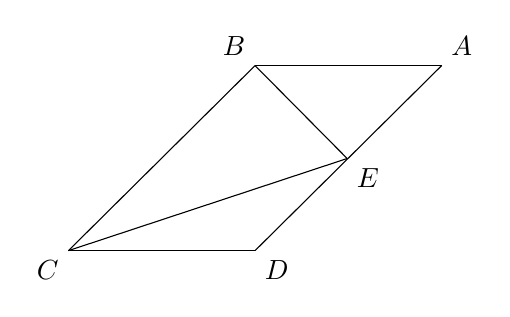
\begin{tikzpicture}
  \coordinate (A) at (5.42,-0.65);
  \coordinate (B) at (3.05,-0.65);
  \coordinate (C) at (0.68,-3.00);
  \coordinate (D) at (3.05,-3.00);
  \coordinate (E) at (4.22,-1.83);

  \draw (B) -- (A);
  \draw (A) -- (D);
  \draw (D) -- (C);
  \draw (C) -- (B);
  \draw (B) -- (E);
  \draw (C) -- (E);

  \node[above left] at (B) {$B$};
  \node[above right] at (A) {$A$};
  \node[below left] at (C) {$C$};
  \node[below right] at (D) {$D$};
  \node[below right] at (E) {$E$};
\end{tikzpicture}
\end{document}
